\documentclass[conference]{IEEEtran}

\usepackage[T1]{fontenc}
\usepackage{lmodern}
\usepackage{cite}
\usepackage{amsmath,amssymb,amsfonts}
\usepackage{algorithmic}
\usepackage{graphicx}
\usepackage{textcomp}
\usepackage{xcolor}
\usepackage{booktabs}
\usepackage{multirow}
\usepackage[hyphens]{url}
\Urlmuskip=0mu plus 2mu\relax
\usepackage{balance}
\usepackage[expansion=false]{microtype}

\sloppy
\emergencystretch=3em

\def\BibTeX{{\rm B\kern-.05em{\sc i\kern-.025em b}\kern-.08em
    T\kern-.1667em\lower.7ex\hbox{E}\kern-.125emX}}

\begin{document}

\title{SCHR-Bench: Evaluating Security-Critical Hallucinations in LLM-Assisted Binary Reverse Engineering via Ground-Truth Mutations}

\author{\IEEEauthorblockN{Anonymous Authors}\\
\IEEEauthorblockA{\textit{Double-Blind Review Copy}}}

\maketitle

\begin{abstract}
Large Language Models (LLMs) are increasingly integrated into software reverse engineering (SRE) workflows to summarize stripped pseudocode and assist analysts in reasoning about binary behavior. However, recent empirical studies reveal that state-of-the-art LLMs frequently struggle with fine-grained semantic logic in stripped binaries: Pordanesh and Tan~\cite{pordanesh2024exploring} reported substantial analyst errors on stealth and persistence routines across decompiled samples, while human--LLM teaming experiments by Basque et al.~\cite{basque2026decompiling} revealed that automated hallucinations severely derail reverse engineering workflows on custom algorithms. Classical evaluation metrics such as BLEU and syntactic recompilability measure surface form rather than whether an LLM detects semantics-inverting code changes. In this paper, we present \textbf{SCHR-Bench}, a controlled pilot benchmark designed to evaluate \textbf{Security-Critical Hallucination Rates (SCHR)} via differential source-level mutations paired with execution-verified ground truth, without executing live malware or requiring commercial IDA Pro licenses. We construct 40 controlled security-decision function pairs ($N = 80$ compiled PE64 variants) spanning five functional categories (Mock Debugger Policy, Toy Byte Decoder, Persistence State Mock, Environment Signal Mock, and Control-Flow \& Boundary Logic) and five binary-adapted mutation operator families ($\mathcal{M}_1$--$\mathcal{M}_5$). All 80 C variants are compiled with MinGW-w64 (\texttt{x86\_64-w64-mingw32-gcc -O2}) and verified across 80 input vectors (160 execution assertions in Experiment E0), confirming that 40/40 pairs diverge on their primary discriminating input vector (Vector 1) and 50/80 total vectors diverge. Across \textbf{1,020 total logged LLM evaluations} ($\tau = 0.0, \text{seed} = 42$)---comprising 540 Layer 1 return-value and explanation runs (480 core CT1--CT3 runs + 60 E4 obfuscation pilot runs in \path{benchmark_raw_logs.json}) and 480 Layer 2 full-factorial paired multiple-choice question (MCQ) runs (\path{benchmark_mcq_logs.json}, $N=80$ per tier across CT1, CT2 with real \texttt{objdump -d -M intel} disassembly, and CT3)---we evaluate \texttt{LLaMA-3.1 8B} and \texttt{Qwen2.5-Coder 14B}. Our results show that: (1) under stripped pseudocode (CT1, $N=80$), \texttt{LLaMA-3.1 8B} exhibits a return-value SCHR of 38.8\% [95\% Wilson CI: 28.8\%, 49.7\%] and an MCQ SCHR of 38.8\% (40.8\% across all 240 MCQ items), whereas \texttt{Qwen2.5-Coder 14B} achieves a return-value SCHR of 23.8\% [15.8\%, 34.1\%] and an MCQ SCHR of 21.2\% (25.0\% across all 240 MCQ items); (2) while 100.0\% (80/80) of stripped CT1 routines pass syntactic C recompilability (\texttt{gcc -fsyntax-only}), pair-level Spearman rank correlation ($\rho \in [+0.293, +0.495]$) confirms that pairs with SCHR errors exhibit higher pairwise BLEU similarity ($\text{BLEU} \in [0.423, 0.584]$) than error-free pairs ($\text{BLEU} \in [0.234, 0.333]$); (3) across both Layer 1 (return-value) and Layer 2 (paired MCQ), passive context escalation to CT2 and CT3 does not yield statistically significant error reductions under McNemar's paired test ($p \in [0.2888, 0.8312]$ at $\alpha = 0.05$); and (4) on a preliminary 5-pair easy-tier pilot subset ($N=10$), combined structural obfuscation (\path{Obf3_Combined}) increases errors by one unit for both models.
\end{abstract}

\begin{IEEEkeywords}
Reverse Engineering, Large Language Models, Hallucination Evaluation, Differential Mutation Testing, Stripped Pseudocode, Code Obfuscation.
\end{IEEEkeywords}

\section{Introduction}
Software Reverse Engineering (SRE) of stripped binary executables is an essential capability in security auditing, vulnerability assessment, and incident response~\cite{shoshitaishvili2016sok,cifuentes1995decompilation}. Because raw assembly instructions impose heavy cognitive load on analysts, operational workflows rely on decompilers such as NSA Ghidra~\cite{ghidra2024nsa} to lift machine code into C-like pseudocode~\cite{yakdan2015norepdb}. Recently, Large Language Models (LLMs) have been widely adopted to summarize decompiled functions, infer variable roles, and explain branch conditions~\cite{pordanesh2024exploring,basque2026decompiling,tan2024llm4decompile,hui2024qwen25coder,dubey2024llama3}.

\begin{figure*}[t]
\centering
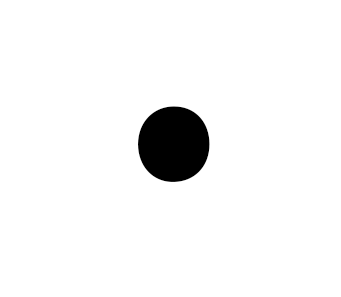
\includegraphics[width=0.94\textwidth]{figures/fig1.png}
\caption{Overview of the SCHR-Bench Evaluation Pipeline: (1) Tier 1 Host GPU Inference Server running Ollama (\texttt{llama3.1:8b} and \texttt{qwen2.5-coder:14b} at $\tau = 0.0, \text{seed} = 42$); and (2) Tier 2 Compilation, Context Generation, and Evaluation Rig executing MinGW-w64 compilation (\texttt{step0\_verify\_e0\_windows.py}), context and real \texttt{objdump -d} assembly construction (\texttt{extract\_contexts.py}), and statistical evaluation (\texttt{step4\_compute\_statistics\_and\_tables.py}). Note: Tier 3 shown in the diagram represents an optional isolated sandbox not used in the quantitative benchmark.}
\label{fig:architecture}
\end{figure*}

However, LLMs remain prone to plausible-sounding \textit{hallucinations}~\cite{ji2023hallucination,min2023factscore}. Empirical evidence highlights the operational severity of this problem in software reverse engineering: in an exploratory study of GPT-4 on decompiled malware subroutines, Pordanesh and Tan~\cite{pordanesh2024exploring} (Table~III, Questions~7--8) observed substantial failure rates on security-critical logic, failing on $46.7\%$ ($7/15$) of stealth techniques and $26.7\%$ ($4/15$) of persistence mechanisms across $n=15$ decompiled samples. Furthermore, in an extensive human-subject study tracking 48 reverse engineers across 109 hours, Basque et al.~\cite{basque2026decompiling} (NDSS 2026) demonstrated that while LLM assistance can accelerate standard library triage, analysts required at least $231\%$ more time on custom algorithms, and unverified vulnerability hallucinations actively degraded analyst comprehension scores by leading practitioners down false diagnostic paths. Similarly, Katpara and Sankaran~\cite{katpara2026firmware} identified the absence of hallucination-specific benchmarks for binary logic as an urgent open research gap.

\textbf{Scope and Benchmarking Strategy:} To construct a reproducible benchmark with deterministic ground truth without executing live malware, requiring commercial IDA Pro licenses, or relying on subjective manual labeling from scratch, we scope \textbf{SCHR-Bench} to x86-64 Windows PE functions under static analysis (NSA Ghidra~\cite{ghidra2024nsa} and GNU \texttt{objdump}) and light-to-moderate structural transformations. While commercial virtualization packers (e.g., VMProtect) destroy decompiler control-flow recovery, SCHR-Bench targets the core dilemma of neural decompilation: measuring whether an LLM notices when a single security-flavored branch condition, cryptographic constant, or state-update operation has been inverted or altered ($f_{\text{orig}}$ vs.\ $f_{\text{mut}}$), and directly contrasting SCHR against surface BLEU and syntactic C recompilability.

We investigate four research questions (RQ1--RQ4) and their corresponding hypotheses (H1--H4): \textbf{RQ1 (H1):} Does the LLM detect single-point security-critical mutations or repeat the unmutated baseline answer? \textbf{RQ2 (H2):} Does SCHR capture semantic inversions that surface BLEU~\cite{papineni2002bleu} and syntactic C recompilability miss? \textbf{RQ3 (H3):} Does appending assembly (CT2) and constant/callee specifications (CT3) reduce SCHR relative to stripped pseudocode (CT1)? \textbf{RQ4 (H4):} How do structural obfuscation templates (\texttt{Obf0}--\texttt{Obf3}) affect SCHR in an exploratory pilot subset ($N=10$)? All code, C sources, compiled PE64 binaries, real \texttt{objdump} disassembly, 240-item paired MCQ gold set, and 1,020 logged runs are available at \url{https://anonymous.4open.science/r/SCHR-Bench-Anon}.

\section{Related Work}

\subsection{Empirical Studies of LLMs in Binary Reverse Engineering}
Table~\ref{tab:guideline_related} summarizes the five foundational studies motivating SCHR-Bench:
\begin{enumerate}
    \item \textbf{Error Rates on Stealth and Evasion (Pordanesh \& Tan, 2024~\cite{pordanesh2024exploring}):} Evaluating GPT-4 across 15 decompiled malware code samples (Table~III, Questions~7--8, pp.~5--6), Pordanesh and Tan reported that error rates rise to \textbf{46.7\% (7/15 samples) on stealth techniques} and \textbf{26.7\% (4/15 samples) on persistence mechanisms}, motivating our focus on security-critical logic.
    \item \textbf{Operational Cost of Hallucinations (Basque et al., NDSS 2026~\cite{basque2026decompiling}):} Across 48 human reverse engineers (109+ hours), Basque et al.\ showed that 3 automated vulnerability hallucinations induced a \textbf{minimum 231\% understanding rate slowdown} (checkpoints per unit time) and consistently misled affected participants into wrong solutions.
    \item \textbf{Adapting Mutation Testing from Hardware HDL to Binary SRE (Qayyum et al., 2025~\cite{qayyum2025verilog}):} Qayyum et al.\ used mutation operators and tiered specification context for \textbf{Verilog HDL} debugging. Because hardware RTL mutations do not apply directly to stripped x86-64 binaries, we design and execution-verify five binary-specific mutation families ($\mathcal{M}_1$--$\mathcal{M}_5$, Section III-D) and adapt context escalation into static binary tiers (CT1--CT4).
    \item \textbf{Atomic Claim Evaluation (Min et al., EMNLP 2023~\cite{min2023factscore}):} FActScore decomposes long-form text into atomic claims; we pair each atomic mutation with an execution-verified return-value oracle and a 240-item full-factorial mutation-aware MCQ gold set.
    \item \textbf{Benchmark Gaps in Malware \& Firmware RE (Katpara \& Sankaran, 2026~\cite{katpara2026firmware}):} Katpara and Sankaran identified the lack of hallucination benchmarks for binary/malware analysis as critical open gaps (Gaps 7 and 8).
\end{enumerate}

\begin{table*}[t]
\centering
\caption{Summary of foundational related literature and how each informs the design of SCHR-Bench.}
\label{tab:guideline_related}
\resizebox{0.98\textwidth}{!}{%
\begin{tabular}{@{}lll@{}}
\toprule
\textbf{Reference} & \textbf{Key Empirical Finding / Method} & \textbf{Role in SCHR-Bench Design} \\
\midrule
Pordanesh \& Tan (2024)~\cite{pordanesh2024exploring} & Reported failure rates on stealth ($7/15$) and persistence ($4/15$) across $n=15$ samples & Direct motivation for measuring SCHR on security-flavored logic \\
Basque et al.\ (NDSS 2026)~\cite{basque2026decompiling} & Controlled human study ($N=48$); $\ge 231\%$ time inflation on custom algorithms; hallucination risks & Demonstrates operational cost of undetected RE hallucinations \\
Qayyum et al.\ (TODAES 2025)~\cite{qayyum2025verilog} & Mutation testing \& tiered context for \textbf{Verilog HDL} debugging & Adapted from Verilog HDL into 5 binary mutation families ($\mathcal{M}_1$--$\mathcal{M}_5$) \& CT1--CT4 \\
Min et al.\ (EMNLP 2023)~\cite{min2023factscore} & \textbf{FActScore}: atomic claim verification of LLM generations & Foundation for atomic mutation-aware MCQ and return-value grading \\
Katpara \& Sankaran (2026)~\cite{katpara2026firmware} & Identifies \textbf{Gaps 7 \& 8}: lack of hallucination benchmarks in binary RE & Positions SCHR-Bench as a controlled ground-truth benchmark \\
\bottomrule
\end{tabular}%
}
\end{table*}

\subsection{Differential Mutation Testing vs.\ Atomic Fact Verification}
Prior evaluations of LLMs in binary reverse engineering have largely focused on atomic claim verification (e.g., assessing whether isolated decompiler assertions or recovered variable types satisfy runtime execution constraints~\cite{pordanesh2024exploring,tan2024llm4decompile}). In contrast, SCHR-Bench introduces \textit{differential pair sensitivity}: rather than evaluating disconnected statements about a single binary, it subjects function pairs ($f_{\text{orig}}$ vs.\ $f_{\text{mut}}$) to single-point semantic mutations with execution-verified ground truth. This directly measures whether an LLM detects security-decision inversions or falls victim to memorized template priors.

\subsection{Decompiler Recovery and Neural Refinement}
Classic decompilers reconstruct high-level control flow from machine code~\cite{cifuentes1995decompilation,yakdan2015norepdb,schwarz2002disassembly}, while DIRE~\cite{lacomis2019dire}, VarBERT~\cite{chen2022varbert}, TREX~\cite{pei2021trex}, LLM4Decompile~\cite{tan2024llm4decompile}, and Wong et al.~\cite{wong2023refining} recover identifier names, variable types, or re-compilable C source. SCHR-Bench complements these works by testing differential semantic sensitivity~\cite{jia2011analysis} under single-point mutations.

\section{The SCHR-Bench Framework}

\subsection{Task Formulation and Metric Definitions}
Let $f_{\text{orig}}$ and $f_{\text{mut}} = \mathcal{M}(f_{\text{orig}})$ denote a pair of original and mutated C functions with signature \texttt{int target(int a, int b, int c)} ($N = 80$ variants across 40 pairs). We evaluate models across two automated layers in \path{code/step3_mcp_server_and_benchmark.py} and \path{code/step4_compute_statistics_and_tables.py}:
\begin{enumerate}
    \item \textbf{Layer 1 --- Concrete Return-Value \& Explanation Task (\texttt{--mode return}, 540 runs):} Given code representation $\mathcal{D}_k(i)$ ($N=80$ per tier across CT1, CT2, CT3, plus 60 E4 obfuscation pilot runs) and discriminating input vector $x_i = (a_i, b_i, c_i)$ (Vector 1 from \path{ground_truth_manifest.json}), the LLM outputs a JSON object with its predicted integer return value $\hat{y}_i \in \mathbb{Z}$ (\path{predicted_return}) and a technical explanation $\mathcal{Y}_i$ (\path{security_interpretation}).
    \item \textbf{Layer 2 --- Full-Factorial Paired Multiple-Choice Gold Set (\texttt{--mode mcq}, 480 runs):} Given $\mathcal{D}_k(i)$ (where CT2 and CT3 include real \texttt{objdump -d -M intel} disassembly from the compiled PE64 binary) and a 4-option question from \path{dataset/gold_set_mcq.json} (240 items per model = 480 total runs: all $N=80$ variants evaluated across all 3 tiers CT1, CT2, and CT3; balanced 60 A, 60 B, 60 C, 60 D, with the longest option correct in 60/240 = 25.0\% of items), the LLM selects option $\hat{c}_i \in \{\text{A, B, C, D}\}$.
\end{enumerate}

We define two primary error metrics:
\begin{enumerate}
    \item \textbf{Security-Critical Hallucination Rate (SCHR):} The proportion of evaluation units ($N=80$) where the model's prediction ($\hat{y}_i$ or $\hat{c}_i$) does not match the execution-verified ground truth ($y_i^*$ or $c_i^*$):
    \begin{equation}
    \text{SCHR} = \frac{1}{N} \sum_{i=1}^N \mathbb{I}\left( \hat{y}_i \neq y_i^* \right)
    \end{equation}
    \item \textbf{Mutant Miss Rate:} Across the $N_{\text{mut}} = 40$ mutated variants, the proportion of mutants on which the LLM predicts the unmutated original return value ($y_{\text{orig}, j}^*$):
    \begin{equation}
    \text{Miss Rate} = \frac{1}{N_{\text{mut}}} \sum_{j=1}^{N_{\text{mut}}} \mathbb{I}\left( \hat{y}_{\text{mut}, j} = y_{\text{orig}, j}^* \right)
    \end{equation}
\end{enumerate}
We compute 95\% confidence intervals $[L, U]$ via the Wilson score interval~\cite{wilson1927probable}:
\begin{equation}
[L, U] = \frac{\hat{p} + \frac{z^2}{2N}}{1 + \frac{z^2}{N}} \pm \frac{z \sqrt{\frac{\hat{p}(1-\hat{p})}{N} + \frac{z^2}{4N^2}}}{1 + \frac{z^2}{N}}
\end{equation}
with $z = 1.96$, and test paired differences between tiers (on the exact same $N=80$ units in both Layer 1 and Layer 2) using McNemar's test~\cite{mcnemar1947note} with continuity correction ($\alpha = 0.05$): $\chi^2 = \frac{(|b - c| - 1)^2}{b + c}$.

\subsection{RQ2 Comparison Metrics: Surface Recompilability vs.\ Pairwise BLEU Detector}
To test Hypothesis H2 (RQ2), we evaluate two complementary dimensions: (1) \textbf{Syntactic C Recompilability} (\path{compute_ct1_recompilability}), which prepends standard decompiler typedefs and stubs to all 80 stripped CT1 routines and tests compilation under \texttt{x86\_64-w64-mingw32-gcc -std=c11 -fsyntax-only} to confirm whether surface validity implies semantic accuracy; and (2) \textbf{Pairwise Explanation Similarity as a Hallucination Detector:} computing 1--3-gram BLEU similarity (\path{simple_bleu_similarity}) between original and mutant explanations ($\mathcal{Y}_{\text{orig}, j}$ vs.\ $\mathcal{Y}_{\text{mut}, j}$) across all 40 pairs to evaluate whether pairwise BLEU functions as a reference-free post-hoc detector for SCHR, quantified via Spearman's rank correlation ($\rho$) and Area Under the ROC Curve (AUROC).

\begin{figure*}[t]
\centering
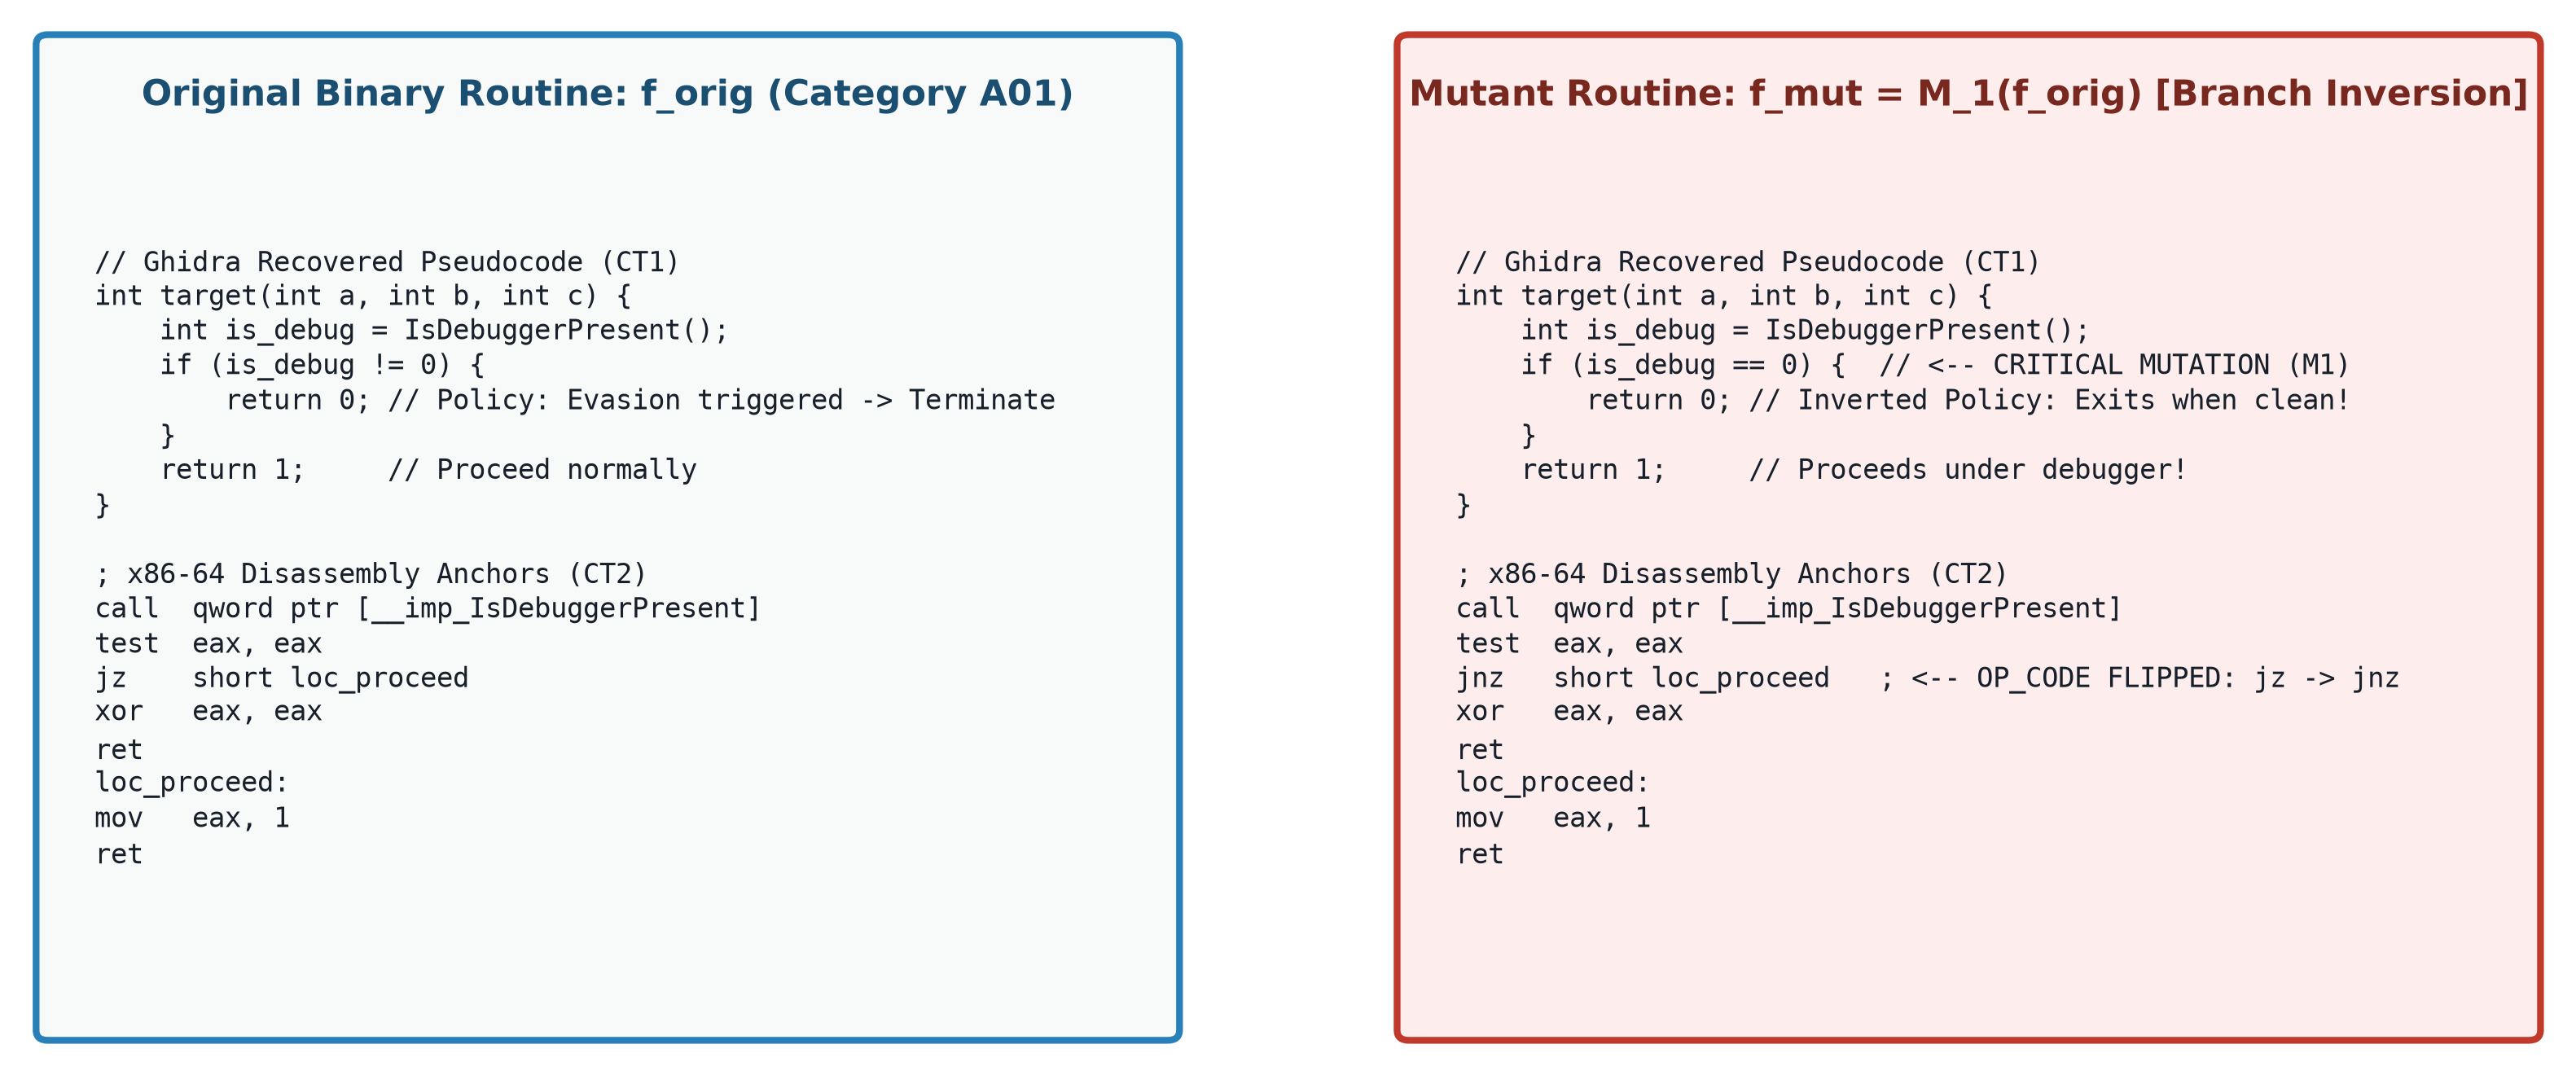
\includegraphics[width=0.92\textwidth]{figures/fig2_decompilation_diff.png}
\caption{Illustrative conceptual diagram of a conditional polarity mutation ($\mathcal{M}_1$: \texttt{!= 0} vs.\ \texttt{== 0}). Note: This figure is an expository illustration containing human-added explanatory annotations (\texttt{/* CRITICAL MUTATION */} and assembly labels \texttt{JZ}/\texttt{JNZ}); the actual prompts evaluated in our benchmark are stripped and contain zero mutation hints.}
\label{fig:decompilation_diff}
\end{figure*}

\subsection{Controlled C Dataset and Context Tiers (CT1--CT4)}
To guarantee operational safety (zero live malware execution or OS registry/service calls), all 40 function pairs (80 C files in \path{dataset/SCHR_Bench_C_Functions/src/}) are implemented as standalone, pure C routines (\texttt{int target(int a, int b, int c)}) across five categories (8 pairs / 16 variants per category; 2 easy, 3 medium, 3 tricky): \textbf{Category A (Mock Debugger Policy --- \texttt{A01}--\texttt{A08})}, \textbf{Category S (Toy Byte Decoder --- \texttt{S01}--\texttt{S08})}, \textbf{Category P (Persistence State Mock --- \texttt{P01}--\texttt{P08})}, \textbf{Category E (Environment Signal Mock --- \texttt{E01}--\texttt{E08})}, and \textbf{Category C (Control-Flow \& Boundary Logic --- \texttt{C01}--\texttt{C08})}.

All 80 C variants are compiled into stripped 64-bit Windows PE executables (\path{dataset/SCHR_Bench_C_Functions/bin/pe_x64_O2/}) and disassembled via \texttt{objdump -d -M intel} (\path{disassembly_objdump_80.json}). In \path{code/extract_contexts.py}, we construct four static context tiers stored in \path{results/decompiled_contexts_80.json}:
\begin{itemize}
    \item \textbf{CT1 (Source-Derived Stripped Pseudocode Template):} Deterministically strips \texttt{target} $\rightarrow$ \path{FUN_140001140}, parameters \texttt{a, b, c} $\rightarrow$ \path{param_1, param_2, param_3}, and static helpers \path{mock_add}/\path{mock_remove} $\rightarrow$ \path{FUN_140001100}/\path{FUN_140001110} inside a standardized Ghidra-style C wrapper.
    \item \textbf{CT2 (+Assembly Anchor):} Appends both the Win64 fastcall register-mapped template (\texttt{ECX}, \texttt{EDX}, \texttt{R8D}) and the real \texttt{objdump -d -M intel} disassembly extracted from the compiled `-O2` PE64 binary (e.g., \texttt{test ecx,ecx; sete al} vs.\ \texttt{setne al}). \textit{Note:} In the initial 540 return-value runs (\path{benchmark_raw_logs.json}), CT2 contained the source-derived register template, whereas in the 480 full-factorial Gold Set MCQ runs (\path{benchmark_mcq_logs.json}) and current \path{decompiled_contexts_80.json}, CT2 and CT3 include the real \texttt{objdump -d -M intel} disassembly.
    \item \textbf{CT3 (+Enriched Constant \& Callee Specifications):} Appends explicit register mappings, hexadecimal-to-decimal immediate lookup tables, and helper specifications. (\textit{Prompt Hygiene Note:} In the initial 540 return-value runs, CT3 and several manifest questions inadvertently included the pair-level \path{semantic_target} descriptor; we subsequently purged \path{semantic_target} from \path{extract_contexts.py} and \path{decompiled_contexts_80.json} and neutralized all 40 questions in \path{ground_truth_manifest.json} prior to running the 480 MCQ evaluations).
    \item \textbf{CT4 (Optional Caller Neighborhood):} Appends the caller harness (\texttt{main} at \path{0x140001200}) and cross-reference context.
\end{itemize}
For Experiment E4 (Section~\ref{sec:rq4}), \path{extract_contexts.py} generates four simulated structural obfuscation templates: \texttt{Obf0} (CT1 baseline), \path{Obf1_CFF} (state-machine \texttt{while(1)} dispatcher), \path{Obf2_Sub} (boolean-arithmetic identity substitution), and \path{Obf3_Combined} (combined dispatcher, substitution, and quadratic predicate).

\subsection{Binary-Adapted Mutation Operators ($\mathcal{M}_1$--$\mathcal{M}_5$) and E0 Verification}
Unlike Verilog HDL mutations~\cite{qayyum2025verilog}, binary reverse engineering requires mutations that survive C compilation into stripped x86-64 machine instructions while altering a security-critical outcome. Table~\ref{tab:operator_mapping} documents the deterministic mapping (\path{OPERATOR_TO_FAMILY_M1_M5} in \path{step4_compute_statistics_and_tables.py}) from the 11 granular \path{mutation_operator} tags in \path{ground_truth_manifest.json} to our five formal mutation families ($\mathcal{M}_1$--$\mathcal{M}_5$).

\begin{table*}[t]
\centering
\caption{Mapping of the 11 manifest \texttt{mutation\_operator} tags across all 40 pairs ($N=80$ variants) to the 5 binary-adapted mutation operator families ($\mathcal{M}_1$--$\mathcal{M}_5$).}
\label{tab:operator_mapping}
\resizebox{0.98\textwidth}{!}{%
\begin{tabular}{@{}lllcc@{}}
\toprule
\textbf{Family} & \textbf{Binary Adaptation \& Security Meaning} & \textbf{Manifest Operator Tags (\texttt{ground\_truth\_manifest.json})} & \textbf{Pairs} & \textbf{Variants} \\
\midrule
$\mathcal{M}_1$ (\textbf{Invert}) & Flips branch polarity (\texttt{JE} $\leftrightarrow$ \texttt{JNE}, \texttt{SETE} $\leftrightarrow$ \texttt{SETNE}) & \texttt{condition\_inversion} (7), \texttt{boolean\_operator} (3), \texttt{condition\_weakening} (1), \texttt{boolean\_precedence} (1) & 12 & 24 \\
$\mathcal{M}_2$ (\textbf{Const})  & Alters immediate XOR keys, bitmasks, or arithmetic shifts & \texttt{constant\_change} (8), \texttt{arithmetic\_operator} (3), \texttt{bitwise\_operator} (1) & 12 & 24 \\
$\mathcal{M}_3$ (\textbf{Swap})   & Swaps state-update effect or callee target (\texttt{OR 1} $\leftrightarrow$ \texttt{AND \textasciitilde 1}) & \texttt{api\_effect\_swap} (4), \texttt{mock\_api\_swap} (1) & 5 & 10 \\
$\mathcal{M}_4$ (\textbf{Bound})  & Shifts strict vs.\ inclusive relational boundary (\texttt{JL} $\leftrightarrow$ \texttt{JLE}) & \texttt{relational\_boundary} (8) & 8 & 16 \\
$\mathcal{M}_5$ (\textbf{Omit})   & Omits a defensive check or state-cleanup operation & \texttt{step\_omission} (3) & 3 & 6 \\
\midrule
\textbf{Total} & \textbf{All 5 Binary-Adapted Mutation Families} & \textbf{All 11 Manifest Tags Verified in E0} & \textbf{40} & \textbf{80} \\
\bottomrule
\end{tabular}%
}
\end{table*}

\textbf{Experiment E0 Execution Verification (\path{step0_verify_e0_windows.py} and \path{tools/check_suite.py}):} Compiling and running all 80 PE64 binaries across both input vectors per pair (80 vectors $\times$ 2 variants = 160 assertions) with \path{x86_64-w64-mingw32-gcc} (v14.2.0, \texttt{-std=c11 -O2 -fno-inline -fno-lto}) confirms that all 160 execution assertions pass (Table~\ref{tab:e0_suite}): \textbf{40/40 pairs (100.0\%)} diverge ($f_{\text{orig}} \neq f_{\text{mut}}$) on \textbf{Vector 1} (the discriminating input queried in the LLM benchmark), and \textbf{50/80 total vectors} diverge.

\begin{table}[t]
\centering
\caption{Experiment E0 Dynamic Binary Execution Verification across all 40 pairs (80 compiled PE64 variants, 160 assertions).}
\label{tab:e0_suite}
\resizebox{0.98\columnwidth}{!}{%
\begin{tabular}{@{}lccccc@{}}
\toprule
\textbf{Category} & \textbf{Pairs (Units)} & \textbf{Diff (E/M/T)} & \textbf{Vecs (Asserts)} & \textbf{Vec 1 Diff} & \textbf{Total Vec Diff} \\
\midrule
\textbf{A: Debug Policy}     & 8 (16) & 2 / 3 / 3 & 16 (32) & \textbf{8/8 (100\%)} & 11/16 \\
\textbf{S: Toy Decoder}      & 8 (16) & 2 / 3 / 3 & 16 (32) & \textbf{8/8 (100\%)} & 9/16  \\
\textbf{P: Persistence Mock} & 8 (16) & 2 / 3 / 3 & 16 (32) & \textbf{8/8 (100\%)} & 12/16 \\
\textbf{E: Env Signal Mock}  & 8 (16) & 2 / 3 / 3 & 16 (32) & \textbf{8/8 (100\%)} & 9/16  \\
\textbf{C: Control Flow}     & 8 (16) & 2 / 3 / 3 & 16 (32) & \textbf{8/8 (100\%)} & 9/16  \\
\midrule
\textbf{Total (SCHR-Bench)}  & \textbf{40 (80)} & \textbf{10 / 15 / 15} & \textbf{80 (160)} & \textbf{40/40 (100\%)} & \textbf{50/80 (62.5\%)} \\
\bottomrule
\end{tabular}%
}
\end{table}

\section{Quantitative Evaluation and Empirical Findings}

\subsection{RQ1: Return-Value and Paired Gold Set MCQ Hallucination Rates ($N=80$)}
Table~\ref{tab:core_results} reports the Layer 1 return-value evaluation across all 80 function variants (480 core runs across CT1--CT3 in \path{results/benchmark_raw_logs.json}), and Table~\ref{tab:mcq_results} reports the Layer 2 full-factorial paired Gold Set MCQ evaluation across all 240 balanced items per model ($N=80$ per tier across CT1, CT2, and CT3; 480 runs in \path{results/benchmark_mcq_logs.json}).

\begin{table*}[t]
\centering
\caption{Layer 1 Core Quantitative Evaluation (Return-Value Oracle, $N=80$ per tier across CT1--CT3 = 480 core runs; together with the 60 E4 obfuscation pilot runs in Table~\ref{tab:obfuscation}, totaling 540 logged Layer 1 runs in \texttt{benchmark\_raw\_logs.json}): SCHR (\%), 95\% Wilson CI, Mutant Miss Rate (\%), Pairwise BLEU (All / Error vs.\ Ok Pairs), Spearman $\rho$ ($p$-value), and Mean Latency.}
\label{tab:core_results}
\resizebox{0.98\textwidth}{!}{%
\begin{tabular}{@{}llcccccccc@{}}
\toprule
\textbf{Model} & \textbf{Context Tier} & \textbf{$N$} & \textbf{Errors} & \textbf{SCHR (\%) [95\% Wilson CI]} & \textbf{Mutant Miss Rate} & \textbf{BLEU (All)} & \textbf{BLEU (Err / Ok)} & \textbf{Spearman $\rho$ ($p$-value)} & \textbf{Latency} \\
\midrule
\texttt{llama3.1:8b}       & \textbf{CT1 (Pseudocode)}  & 80 & 31 & \textbf{38.8\%} [28.8\%, 49.7\%] & 32.5\% (13/40) & 0.376 & 0.423 / 0.234 & $+0.326$ ($p=0.0335$) & 6.93s \\
\texttt{llama3.1:8b}       & \textbf{CT2 (+Pseudo-Asm)} & 80 & 29 & \textbf{36.2\%} [26.6\%, 47.2\%] & 27.5\% (11/40) & 0.400 & 0.457 / 0.282 & $+0.324$ ($p=0.0347$) & 7.33s \\
\texttt{llama3.1:8b}       & \textbf{CT3 (+Enriched)}   & 80 & 28 & \textbf{35.0\%} [25.5\%, 45.9\%] & 27.5\% (11/40) & 0.462 & 0.532 / 0.333 & $+0.293$ ($p=0.0593$) & 7.53s \\
\midrule
\texttt{qwen2.5-coder:14b} & \textbf{CT1 (Pseudocode)}  & 80 & 19 & \textbf{23.8\%} [15.8\%, 34.1\%] & 27.5\% (11/40) & 0.358 & 0.497 / 0.256 & $+0.399$ ($p=0.0073$) & 26.69s \\
\texttt{qwen2.5-coder:14b} & \textbf{CT2 (+Pseudo-Asm)} & 80 & 16 & \textbf{20.0\%} [12.7\%, 30.0\%] & 25.0\% (10/40) & 0.403 & 0.584 / 0.294 & $+0.495$ ($p=0.0004$) & 26.77s \\
\texttt{qwen2.5-coder:14b} & \textbf{CT3 (+Enriched)}   & 80 & 15 & \textbf{18.8\%} [11.7\%, 28.7\%] & 25.0\% (10/40) & 0.409 & 0.582 / 0.315 & $+0.475$ ($p=0.0009$) & 26.31s \\
\bottomrule
\end{tabular}%
}
\end{table*}

\begin{table*}[t]
\centering
\caption{Layer 2 Full-Factorial Paired Gold Set MCQ Evaluation (\texttt{dataset/gold\_set\_mcq.json}, $N=80$ per tier, 240 items per model = 480 runs, incorporating real \texttt{objdump -d -M intel} disassembly in CT2 and CT3).}
\label{tab:mcq_results}
\resizebox{0.98\textwidth}{!}{%
\begin{tabular}{@{}llccccccc@{}}
\toprule
\textbf{Model} & \textbf{Paired Context Tier ($N=80$)} & \textbf{Items ($N$)} & \textbf{Correct} & \textbf{Errors} & \textbf{MCQ SCHR (\%) [95\% Wilson CI]} & \textbf{Accuracy (\%)} & \textbf{McNemar vs.\ CT1 ($b/c, p$)} & \textbf{Mean Latency} \\
\midrule
\texttt{llama3.1:8b}       & CT1 (Stripped Pseudocode Baseline)      & 80           & 49           & 31          & \textbf{38.8\%} [28.8\%, 49.7\%] & 61.3\%          & ---                        & 1.10s \\
\texttt{llama3.1:8b}       & CT2 (+Real \texttt{objdump -d} Assembly) & 80          & 44           & 36          & \textbf{45.0\%} [34.6\%, 55.9\%] & 55.0\%          & $b=9, c=14$ ($p=0.4042$)   & 1.56s \\
\texttt{llama3.1:8b}       & CT3 (+Real \texttt{objdump -d} \& Spec)  & 80          & 49           & 31          & \textbf{38.8\%} [28.8\%, 49.7\%] & 61.3\%          & $b=11, c=11$ ($p=0.8312$)  & 1.76s \\
\texttt{llama3.1:8b}       & \textbf{All Gold Set Items (CT1--CT3)} & \textbf{240} & \textbf{142} & \textbf{98} & \textbf{40.8\%} [34.8\%, 47.1\%] & \textbf{59.2\%} & ---                        & 1.47s \\
\midrule
\texttt{qwen2.5-coder:14b} & CT1 (Stripped Pseudocode Baseline)      & 80           & 63           & 17          & \textbf{21.2\%} [13.7\%, 31.4\%] & 78.8\%          & ---                        & 3.38s \\
\texttt{qwen2.5-coder:14b} & CT2 (+Real \texttt{objdump -d} Assembly) & 80          & 59           & 21          & \textbf{26.2\%} [17.9\%, 36.8\%] & 73.8\%          & $b=6, c=10$ ($p=0.4533$)   & 5.09s \\
\texttt{qwen2.5-coder:14b} & CT3 (+Real \texttt{objdump -d} \& Spec)  & 80          & 58           & 22          & \textbf{27.5\%} [18.9\%, 38.1\%] & 72.5\%          & $b=7, c=12$ ($p=0.3588$)   & 5.04s \\
\texttt{qwen2.5-coder:14b} & \textbf{All Gold Set Items (CT1--CT3)} & \textbf{240} & \textbf{180} & \textbf{60} & \textbf{25.0\%} [19.9\%, 30.8\%] & \textbf{75.0\%} & ---                        & 4.51s \\
\midrule
\textbf{Random Guessing Baseline} & 4-Option Chance Baseline & \textbf{240} & \textbf{60} & \textbf{180} & \textbf{75.0\%} [69.2\%, 80.0\%] & \textbf{25.0\%} & ---                        & --- \\
\bottomrule
\end{tabular}%
}
\end{table*}

Under stripped pseudocode (CT1, $N=80$), Layer 1 (return-value) and Layer 2 (paired MCQ) yield virtually identical baseline hallucination rates: \path{llama3.1:8b} records \textbf{38.8\%} (31/80) in return-value mode and \textbf{38.8\%} (31/80) in CT1 MCQ mode (overall 240-item MCQ SCHR: \textbf{40.8\%}), while \path{qwen2.5-coder:14b} records \textbf{23.8\%} (19/80) in return-value mode and \textbf{21.2\%} (17/80) in CT1 MCQ mode (overall 240-item MCQ SCHR: \textbf{25.0\%}). For reference, a naive random guess across 4 options yields a $75.0\%$ error rate ($25.0\%$ accuracy). Both models perform significantly better than chance ($38.8\%\text{--}45.0\%$ SCHR for LLaMA-3.1; $21.2\%\text{--}27.5\%$ for Qwen2.5-Coder), confirming that models comprehend general code structure but fail specifically on fine-grained mutation semantics.

Tables~\ref{tab:category_matrix} and \ref{tab:central_matrix} disaggregate Layer 1 SCHR across the five functional categories ($n=16$ per category) and five mutation families ($\mathcal{M}_1$--$\mathcal{M}_5$, $N=80$). Both models exhibit their highest failure rates on Category S (Toy Byte Decoders: 56.2\%--62.5\%) and $\mathcal{M}_2$ (Constant \& Arithmetic Alteration: 50.0\% at CT1), while \path{qwen2.5-coder:14b} achieves lower error rates on $\mathcal{M}_1$ Condition Inversion (20.8\% vs.\ 50.0\% on LLaMA-3.1 at CT1) and Category P Persistence Mocks (0.0\% at CT2/CT3).

\textbf{Persistent Template Inertia in Category S (Toy Byte Decoders):} As detailed in Table~\ref{tab:category_matrix}, Category S exhibits the highest and most persistent SCHR across all tiers and models ($56.2\%\text{--}62.5\%$). Trace analysis of LLM reasoning chains reveals that toy byte decoders (e.g., rolling XOR keys, table-lookup decoders) heavily trigger LLM pre-training memorization: upon encountering loop-based decoding idioms, models reflexively produce generalized textbook explanations while ignoring subtle mutations in byte constants, step sizes, or terminal loop conditions.

\begin{table*}[t]
\centering
\caption{Domain-Specific SCHR (\%) Breakdown across the 5 Functional Categories A, S, P, E, C ($n=16$ variants per category, $N=80$ total).}
\label{tab:category_matrix}
\resizebox{0.96\textwidth}{!}{%
\begin{tabular}{@{}llccccc@{}}
\toprule
\textbf{Model} & \textbf{Context Tier} & \textbf{A: Debug Policy} & \textbf{S: Toy Decoder} & \textbf{P: Persistence Mock} & \textbf{E: Env Signal} & \textbf{C: Control Flow} \\
\midrule
\texttt{llama3.1:8b}       & \textbf{CT1 (Pseudocode)}  & 43.8\% (7/16) & 56.2\% (9/16)  & 12.5\% (2/16) & 43.8\% (7/16) & 37.5\% (6/16) \\
\texttt{llama3.1:8b}       & \textbf{CT2 (+Pseudo-Asm)} & 31.2\% (5/16) & 62.5\% (10/16) & 6.2\% (1/16)  & 50.0\% (8/16) & 31.2\% (5/16) \\
\texttt{llama3.1:8b}       & \textbf{CT3 (+Enriched)}   & 31.2\% (5/16) & 62.5\% (10/16) & 6.2\% (1/16)  & 43.8\% (7/16) & 31.2\% (5/16) \\
\midrule
\texttt{qwen2.5-coder:14b} & \textbf{CT1 (Pseudocode)}  & 12.5\% (2/16) & 56.2\% (9/16)  & 12.5\% (2/16) & 18.8\% (3/16) & 18.8\% (3/16) \\
\texttt{qwen2.5-coder:14b} & \textbf{CT2 (+Pseudo-Asm)} & 6.2\% (1/16)  & 56.2\% (9/16)  & \textbf{0.0\% (0/16)} & 18.8\% (3/16) & 18.8\% (3/16) \\
\texttt{qwen2.5-coder:14b} & \textbf{CT3 (+Enriched)}   & 6.2\% (1/16)  & 56.2\% (9/16)  & \textbf{0.0\% (0/16)} & 18.8\% (3/16) & 12.5\% (2/16) \\
\bottomrule
\end{tabular}%
}
\end{table*}

\begin{table*}[t]
\centering
\caption{Central Evaluation Matrix (E1--E3): SCHR (\%) across Mutation Operator Families ($\mathcal{M}_1$--$\mathcal{M}_5$, $N=80$).}
\label{tab:central_matrix}
\resizebox{0.96\textwidth}{!}{%
\begin{tabular}{@{}llcccccc@{}}
\toprule
\textbf{Model} & \textbf{Context Tier} & \textbf{$\mathcal{M}_1$: Invert ($n=24$)} & \textbf{$\mathcal{M}_2$: Const ($n=24$)} & \textbf{$\mathcal{M}_3$: Swap ($n=10$)} & \textbf{$\mathcal{M}_4$: Bound ($n=16$)} & \textbf{$\mathcal{M}_5$: Omit ($n=6$)} & \textbf{Overall SCHR} \\
\midrule
\texttt{llama3.1:8b}       & \textbf{CT1 (Pseudocode)}  & 50.0\% (12/24) & 50.0\% (12/24) & 10.0\% (1/10) & 31.2\% (5/16) & 16.7\% (1/6) & \textbf{38.8\%} (31/80) \\
\texttt{llama3.1:8b}       & \textbf{CT2 (+Pseudo-Asm)} & 33.3\% (8/24)  & 54.2\% (13/24) & 10.0\% (1/10) & 31.2\% (5/16) & 33.3\% (2/6) & \textbf{36.2\%} (29/80) \\
\texttt{llama3.1:8b}       & \textbf{CT3 (+Enriched)}   & 33.3\% (8/24)  & 54.2\% (13/24) & 0.0\% (0/10)  & 31.2\% (5/16) & 33.3\% (2/6) & \textbf{35.0\%} (28/80) \\
\midrule
\texttt{qwen2.5-coder:14b} & \textbf{CT1 (Pseudocode)}  & 20.8\% (5/24)  & 50.0\% (12/24) & 10.0\% (1/10) & 6.2\% (1/16)  & 0.0\% (0/6)  & \textbf{23.8\%} (19/80) \\
\texttt{qwen2.5-coder:14b} & \textbf{CT2 (+Pseudo-Asm)} & 12.5\% (3/24)  & 45.8\% (11/24) & 0.0\% (0/10)  & 12.5\% (2/16) & 0.0\% (0/6)  & \textbf{20.0\%} (16/80) \\
\texttt{qwen2.5-coder:14b} & \textbf{CT3 (+Enriched)}   & 12.5\% (3/24)  & 41.7\% (10/24) & 0.0\% (0/10)  & 12.5\% (2/16) & 0.0\% (0/6)  & \textbf{18.8\%} (15/80) \\
\bottomrule
\end{tabular}%
}
\end{table*}

\subsection{RQ2: Surface Metric Blindness and Pairwise BLEU as a Cheap Hallucination Detector}
Our empirical findings reveal two critical insights regarding surface metrics and semantic fidelity (supporting H2): (1) \textbf{100.0\% Syntactic C Recompilability (80/80):} Verified via \path{compute_ct1_recompilability} (\texttt{x86\_64-w64-mingw32-gcc -std=c11 -fsyntax-only}), every stripped CT1 routine (including all 40 mutated variants) compiles cleanly with zero syntax errors (omitted as a redundant table column because all 80/80 variants pass identically across every row), proving that syntactic compilability does not imply semantic correctness; and (2) \textbf{Pairwise Explanation Similarity as a Cheap Post-Hoc Detector:} Pairs with SCHR errors exhibit higher pairwise BLEU similarity than error-free pairs ($0.423$ vs.\ $0.234$ on LLaMA CT1, $\rho = +0.326, p = 0.0335$; $0.497$ vs.\ $0.256$ on Qwen CT1, $\rho = +0.399, p = 0.0073$; and $\rho = +0.495, p = 0.0004$ on Qwen CT2), because models generate nearly identical boilerplate explanations when they suffer from semantic inertia. Consequently, treating pairwise explanation similarity as a threshold classifier for SCHR achieves an \textbf{AUROC of 0.683} on \path{llama3.1:8b} and up to \textbf{0.811} on \path{qwen2.5-coder:14b} (CT2), demonstrating that pairwise explanation consistency serves as an effective, reference-free screening mechanism for silent hallucinations.

\subsection{RQ3: Context Escalation, Statistical Power, and Cross-Tier Regressions}
\label{sec:rq3}
Because Layer 2 evaluates all $N=80$ variants under full-factorial paired MCQ conditions with real \texttt{objdump -d -M intel} disassembly (Table~\ref{tab:mcq_results}), it provides our primary benchmark for cross-tier comparisons. (As noted in Section~\ref{sec:threats}, the initial Layer 1 return-value CT3 prompt contained prompt metadata confounding, so Layer 1 comparisons are presented for historical context while Layer 2 serves as the clean reference).

In Layer 2 MCQ (Table~\ref{tab:mcq_results}), error rates remain persistent across tiers: $38.8\%$ (CT1) $\rightarrow 45.0\%$ (CT2) $\rightarrow 38.8\%$ (CT3) on LLaMA-3.1; $21.2\%$ (CT1) $\rightarrow 26.2\%$ (CT2) $\rightarrow 27.5\%$ (CT3) on Qwen2.5-Coder. Paired McNemar tests confirm no statistically significant difference relative to CT1 ($p \in [0.3588, 0.8312]$). However, we highlight two key nuances: (1) \textbf{Statistical Power Constraints:} Because discordant pairs are modest ($b, c \in [6, 14]$ on $N=80$), McNemar's test has limited statistical power, indicating \textit{insufficient empirical evidence to claim an effect} rather than proving context escalation is entirely ineffective; and (2) \textbf{Assembly-Induced Regressions on Boundary Logic:} On LLaMA-3.1, appending real assembly (CT2) increased SCHR from $38.8\%$ to $45.0\%$ ($b=9$ recoveries vs.\ $c=14$ regressions, $p=0.4042$) due to cognitive distraction from verbose x86-64 assembly listings on basic arithmetic inequalities ($\mathcal{M}_2$) and boundary checks.

\begin{table}[t]
\centering
\caption{McNemar's Paired Test on Layer 1 Return-Value comparing CT1 vs.\ CT2/CT3 ($N=80, \alpha=0.05$). $b$: CT1 Err $\rightarrow$ Fix; $c$: CT1 Ok $\rightarrow$ Err.}
\label{tab:mcnemar}
\resizebox{0.98\columnwidth}{!}{%
\begin{tabular}{@{}llcccccc@{}}
\toprule
\textbf{Model} & \textbf{Comparison} & \textbf{$b$} & \textbf{$c$} & \textbf{Net} & \textbf{$\chi^2$} & \textbf{$p$-val} & \textbf{Significance ($\alpha=0.05$)} \\
\midrule
\texttt{llama3.1} & \textbf{CT1 vs.\ CT2} & 6 & 4 & $+2$ & 0.100 & 0.7518 & Not sig.\ ($p \ge 0.05$) \\
\texttt{llama3.1} & \textbf{CT1 vs.\ CT3} & 8 & 5 & $+3$ & 0.308 & 0.5791 & Not sig.\ ($p \ge 0.05$) \\
\midrule
\texttt{qwen2.5}  & \textbf{CT1 vs.\ CT2} & 5 & 2 & $+3$ & 0.571 & 0.4497 & Not sig.\ ($p \ge 0.05$) \\
\texttt{qwen2.5}  & \textbf{CT1 vs.\ CT3} & 6 & 2 & $+4$ & 1.125 & 0.2888 & Not sig.\ ($p \ge 0.05$) \\
\bottomrule
\end{tabular}%
}
\end{table}

\begin{figure}[t]
\centering
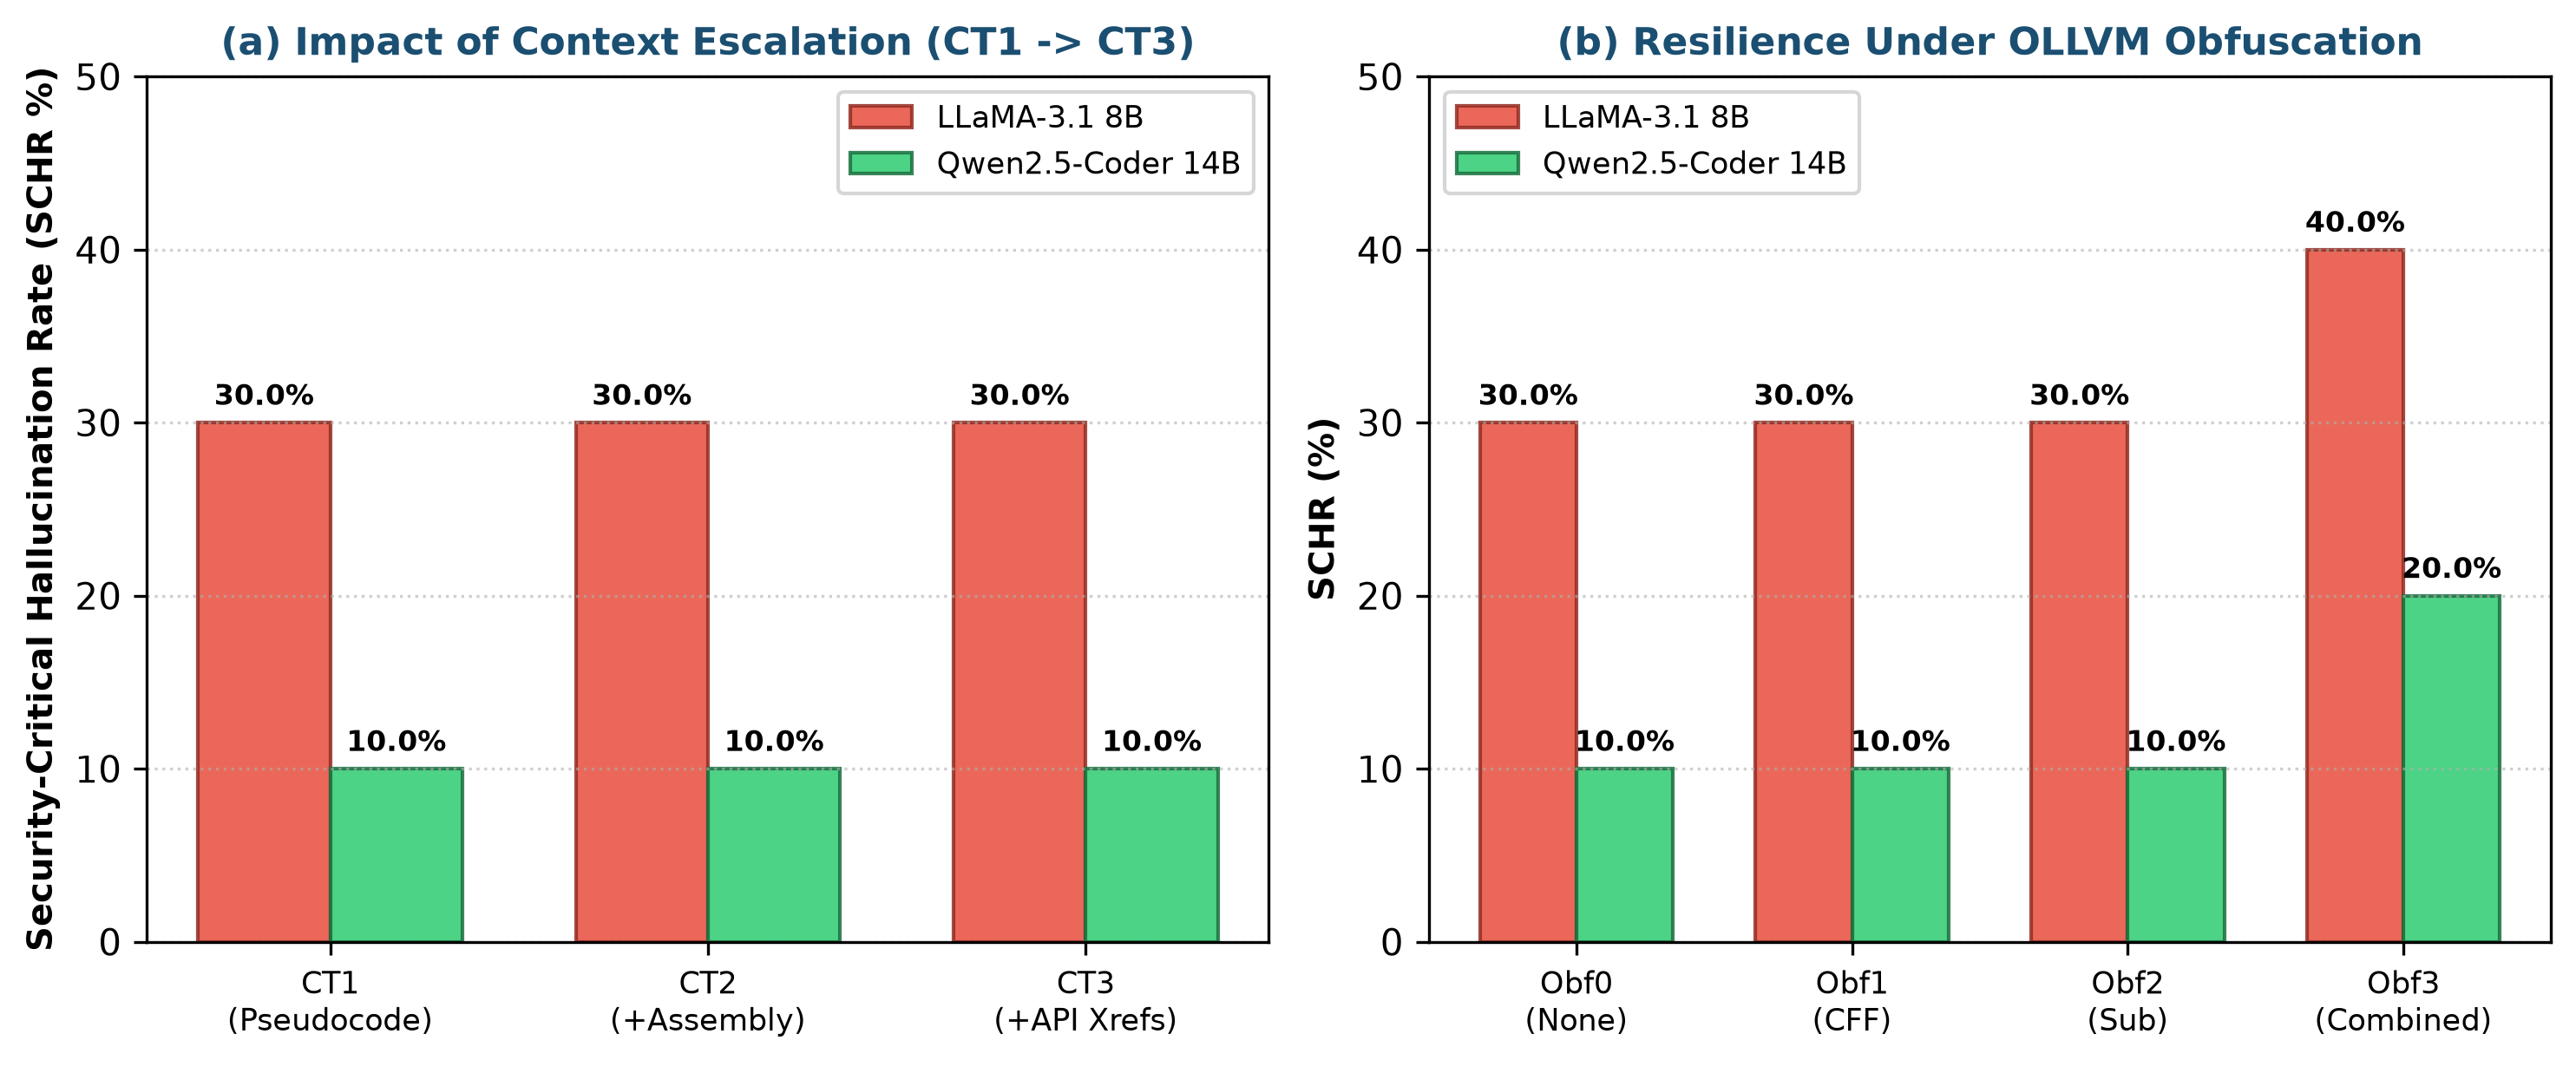
\includegraphics[width=0.98\columnwidth]{figures/fig3_empirical_schr.png}
\caption{Empirical SCHR (\%) across Context Tiers CT1--CT3 ($N=80$ variants) and Simulated Structural Obfuscation Templates \texttt{Obf0}--\texttt{Obf3} ($N=10$ easy-tier pilot subset).}
\label{fig:empirical_schr}
\end{figure}

\subsection{Preliminary Pilot Observations on Structural Obfuscation ($N=10$ Pilot Subset)}
\label{sec:rq4}
In Experiment E4, we conducted an exploratory pilot study evaluating both models across four simulated structural obfuscation templates (\texttt{Obf0}--\texttt{Obf3}) on a 5-pair easy-tier pilot subset (\texttt{A01}, \texttt{S01}, \texttt{P01}, \texttt{E01}, \texttt{C01}; $N=10$ variants, 60 runs in \path{benchmark_raw_logs.json}). As shown in Table~\ref{tab:obfuscation}, isolated \path{Obf1_CFF} or \path{Obf2_Sub} leaves error counts unchanged relative to \texttt{Obf0} (3/10 on LLaMA-3.1; 1/10 on Qwen2.5-Coder), whereas \path{Obf3_Combined} results in one additional error for each model ($3/10 \rightarrow 4/10$ on LLaMA-3.1; $1/10 \rightarrow 2/10$ on Qwen2.5-Coder). We explicitly emphasize that $N=10$ yields wide Wilson confidence intervals ($[16.8\%, 68.7\%]$ for $4/10$); hence, these findings are presented strictly as \textbf{preliminary pilot observations} rather than primary contributions. A full-scale evaluation across all 80 variants compiled with real OLLVM passes~\cite{junod2015ollvm} is deferred to future work.

\begin{table}[t]
\centering
\caption{Experiment E4 (RQ4): Preliminary evaluation of simulated obfuscation templates (\texttt{Obf0}--\texttt{Obf3}) on the 5-pair easy-tier pilot subset ($N=10$ variants; 20 CT1 baseline runs + 60 obfuscated \texttt{Obf1}--\texttt{Obf3} runs = 540 total Layer 1 runs in \texttt{benchmark\_raw\_logs.json}).}
\label{tab:obfuscation}
\resizebox{0.98\columnwidth}{!}{%
\begin{tabular}{@{}llccc@{}}
\toprule
\textbf{Model} & \textbf{Simulated Template} & \textbf{Pilot $N$} & \textbf{Errors} & \textbf{SCHR [95\% Wilson CI]} \\
\midrule
\texttt{llama3.1:8b}   & Obf0 (CT1 Baseline) & 10 & 3 & 30.0\% [10.8\%, 60.3\%] \\
\texttt{llama3.1:8b}   & Obf1\_CFF (Wrapper) & 10 & 3 & 30.0\% [10.8\%, 60.3\%] \\
\texttt{llama3.1:8b}   & Obf2\_Sub (Identity) & 10 & 3 & 30.0\% [10.8\%, 60.3\%] \\
\texttt{llama3.1:8b}   & Obf3\_Combined & 10 & 4 & 40.0\% [16.8\%, 68.7\%] \\
\midrule
\texttt{qwen2.5-coder} & Obf0 (CT1 Baseline) & 10 & 1 & 10.0\% [1.8\%, 40.4\%] \\
\texttt{qwen2.5-coder} & Obf1\_CFF (Wrapper) & 10 & 1 & 10.0\% [1.8\%, 40.4\%] \\
\texttt{qwen2.5-coder} & Obf2\_Sub (Identity) & 10 & 1 & 10.0\% [1.8\%, 40.4\%] \\
\texttt{qwen2.5-coder} & Obf3\_Combined & 10 & 2 & 20.0\% [5.7\%, 51.0\%] \\
\bottomrule
\end{tabular}%
}
\end{table}

\section{Breakdown of Logged CT1 Failures by Mutation Mechanism}
Across the 160 Layer 1 CT1 evaluations (80 variants $\times$ 2 models), exactly \textbf{50 return-value prediction errors} occurred (31 on \path{llama3.1:8b} and 19 on \path{qwen2.5-coder:14b}). Table~\ref{tab:error_taxonomy} deterministically groups all 50 logged CT1 failures according to the objective \path{mutation_operator} tag in \path{ground_truth_manifest.json}: Constant \& Arithmetic Alteration ($\mathcal{M}_2$) accounts for 48.0\% (24/50), Condition \& Boolean Inversion ($\mathcal{M}_1$) accounts for 34.0\% (17/50), Relational Boundary Shift ($\mathcal{M}_4$) accounts for 12.0\% (6/50), and Target Swap / Step Omission ($\mathcal{M}_3, \mathcal{M}_5$) accounts for 6.0\% (3/50).

\begin{table}[t]
\centering
\caption{Deterministic grouping of all 50 logged CT1 errors by ground-truth mutation operator family in \texttt{results/benchmark\_raw\_logs.json}.}
\label{tab:error_taxonomy}
\resizebox{0.98\columnwidth}{!}{%
\begin{tabular}{@{}lccc@{}}
\toprule
\textbf{Mutation Mechanism Group} & \textbf{LLaMA ($n=31$)} & \textbf{Qwen ($n=19$)} & \textbf{Total ($N=50$)} \\
\midrule
\textbf{Constant \& Arithmetic ($\mathcal{M}_2$)} & 12 & 12 & \textbf{24 (48.0\%)} \\
\textbf{Condition \& Boolean ($\mathcal{M}_1$)}   & 12 & 5  & \textbf{17 (34.0\%)} \\
\textbf{Relational Boundary ($\mathcal{M}_4$)}    & 5  & 1  & \textbf{6 (12.0\%)}  \\
\textbf{Target Swap \& Omit ($\mathcal{M}_3, \mathcal{M}_5$)} & 2  & 1  & \textbf{3 (6.0\%)}   \\
\bottomrule
\end{tabular}%
}
\end{table}

\section{Safety, Threats to Validity, and Conclusion}

\subsection{Ethical and Operational Safety}
A primary advantage of SCHR-Bench is its strict adherence to static analysis safety: all 80 benchmark variants are self-contained, pure C functions (\texttt{int target(int a, int b, int c)}) containing zero live malware payloads and zero destructive OS calls. No live malware samples are distributed or executed in our repository.

\subsection{Threats to Validity and Scope Limitations}
\label{sec:threats}
We explicitly document the scope boundaries and limitations of our current study:
\begin{enumerate}
    \item \textbf{Mock C Functions vs.\ Real Malware and Live Win32 APIs:} Our 40 function pairs are self-contained mock routines (using static helpers \path{mock_add}/\path{mock_remove} rather than live Win32 APIs such as \texttt{RegSetValueEx} or \texttt{IsDebuggerPresent}) with one mutation per function pair. Thus, SCHR on our controlled suite represents a lower bound on the difficulty of real-world malware reverse engineering.
    \item \textbf{Source-Derived Pseudocode and Obfuscation Templates vs.\ Full Ghidra/OLLVM Builds:} While all 80 variants are compiled to stripped PE64 binaries and disassembled with real \texttt{objdump -d -M intel} (used in our 480 paired Gold Set MCQ runs and linked in \path{decompiled_contexts_80.json}), the CT1 pseudocode and \texttt{Obf1}--\texttt{Obf3} templates are generated deterministically from C source by \path{extract_contexts.py} rather than lifted via Ghidra Headless or compiled with OLLVM passes~\cite{junod2015ollvm}. Moreover, Experiment E4 evaluates only an $N=10$ easy-tier pilot subset.
    \item \textbf{Automated Return-Value \& MCQ Grading vs.\ Dual-Rater Free-Form Cohen's $\kappa$:} To guarantee deterministic reproducibility, our 1,020 logged runs rely on exact return-value matching (540 runs) and 4-option MCQ matching (480 runs). While we provide the free-form atomic claim prompt (\path{prompts/explanation_system_prompt.txt}), dual-annotator human grading of free-text explanations with Cohen's $\kappa$~\cite{cohen1960coefficient} was not conducted in this phase.
    \item \textbf{Prompt Metadata Confounding in Initial Return-Value CT3 Logs:} In the initial 540 return-value runs, the CT3 template and several manifest questions inadvertently included the pair-level \path{semantic_target} string; this was fully removed in \path{extract_contexts.py}, \path{ground_truth_manifest.json}, and the 480 Gold Set MCQ evaluations.
    \item \textbf{Model \& Decoding Coverage:} We evaluated two open-weight models (\texttt{llama3.1:8b} and \texttt{qwen2.5-coder:14b}) locally via Ollama at $\tau = 0.0$ (\texttt{seed=42}) rather than commercial cloud APIs or multi-seed $\tau > 0$ sampling.
\end{enumerate}

\subsection{Future Work and Conclusion}
\textbf{Future Work:} We plan to: (1) run Ghidra Headless decompilation and real OLLVM compiler passes across all 80 binaries; (2) conduct dual-annotator FActScore claim grading with Cohen's $\kappa$ on free-form explanations and compare against commercial API models; and (3) evaluate active mitigation architectures such as \textit{Interleaved Chain-of-Thought (CoT) Register Tracing} and \textit{Multi-Engine Decompiler Verification (E6)}.

\textbf{Conclusion:} We presented \textbf{SCHR-Bench}, a controlled differential mutation benchmark measuring whether LLMs detect security-critical behavioral changes across 40 original/mutant C function pairs ($N=80$ execution-verified PE64 variants, 1,020 total logged evaluations across return-value and full-factorial paired Gold Set MCQ tasks). Our results show that \texttt{LLaMA-3.1 8B} and \texttt{Qwen2.5-Coder 14B} exhibit baseline CT1 error rates of 38.8\% and 23.8\% (and overall 240-item Gold Set MCQ SCHR of 40.8\% and 25.0\%), that 100.0\% syntactic recompilability and high pairwise BLEU ($\rho \in [+0.293, +0.495]$) mask semantic inversions, and that passive context escalation (CT2/CT3) provides non-significant changes under McNemar's test ($p \ge 0.2888$). All artifacts are publicly available at \url{https://anonymous.4open.science/r/SCHR-Bench-Anon}.

\section*{Disclosure of AI Usage}
During the preparation of this project under the IAM302t Research-Based Learning (RBL) curriculum, the authors used local LLMs (\texttt{LLaMA-3.1 8B} and \texttt{Qwen2.5-Coder 14B} via Ollama) as the subjects of empirical evaluation, and used AI coding/writing assistance for LaTeX formatting, script refactoring, and language polishing. All experimental scripts, C source functions, and statistical tables were verified by the authors.

\balance
\bibliographystyle{IEEEtran}
\bibliography{references}

\end{document}
